\documentclass[a4paper,10pt]{article}
%
%--------------------   start of the 'preamble'
%
\usepackage{graphicx,amssymb,amstext,amsmath}
\usepackage[usenames,dvipsnames]{color}% enable colors
\usepackage{xcolor}                    % other colors
\usepackage{xspace}
\usepackage{wasysym}
\usepackage{hyperref}
\usepackage{float}
\usepackage{slashbox}
\usepackage{verbatim}
\usepackage{listings}                  % enable code writings
\usepackage{appendix}
%
%---------------------   end of the 'preamble'
%
%--------------------   Define new commands
%
\newcommand{\tel}{\textbf{TELEMAC}\xspace}
\newcommand{\teld}{\textbf{TELEMAC-2D}\xspace} 
\newcommand{\stb}{\textbf{STBTEL}\xspace}
\newcommand{\teldd}{\textbf{TELEMAC-3D}\xspace}
\newcommand{\bief}{\textbf{BIEF}\xspace}
\newcommand{\estel}{\textbf{ESTEL}\xspace}
\newcommand{\slf}{\textbf{SELAFIN}\xspace}
\newcommand{\sal}{\textbf{SALOME}\xspace}
\newcommand{\unv}{\textbf{UNV}\xspace}
\newcommand{\med}{\textbf{MED}\xspace}
\newcommand{\vtk}{\textbf{VTK}\xspace}
\newcommand{\cgns}{\textbf{CGNS}\xspace}
\newcommand{\tecplot}{\textbf{TECPLOT}\xspace}
\newcommand{\hdf}{\textbf{HDF5}\xspace}
\newcommand{\todo}[1]{\textcolor{red}{TODO: #1}\\} % macro for todo entries
% New gray color
\definecolor{LightGray}{gray}{0.95}
\newcommand{\codebash}[1]{
  \lstset{
    language=bash,
    breaklines=true,
    inputencoding=utf8,
    numbers=left, 
    firstnumber=0,
    numberstyle=\footnotesize,
    stepnumber=5,             
    basicstyle=\ttfamily, 
    showspaces=false,
    showstringspaces=false,
    showtabs=false,
    frame=single,
    commentstyle=\itshape\color{Purple},
    stringstyle=\color{NavyBlue},
    keywordstyle=\color{Maroon},
    morestring=[b]',
    backgroundcolor=\color{LightGray}
  }
  \lstinputlisting{#1}
}


%
%-----------------------------------------------------------
\begin{document}
%-----------------------------------------------------------
\title{Implementation of new Format Converters in \stb}
\author{Yoann AUDOUIN, Charles MOULINEC, David EMERSON}


\maketitle
%-----------------------------------------------------------
\begin{abstract}
This document analyses the format converters already existing in \stb v6p0 (from 
(SUPERTAB6, SUPERTAB4, MASTER2, SIMAIL, SELAFIN, TRIGRID, FASTTABS) to \slf).
More format converters are implemented to be able to
go from (\med, \unv, \slf, \cgns) to (\med, \unv, \slf, \vtk, \cgns) by using a custom Fortran object as go-between.
\end{abstract}
\vfill
EDF Contacts: \\
Fabien DECUNG, Christophe DENIS, Emile RAZAFINDRAKOTO
\newpage
%-----------------------------------------------------------

\section{Introduction}
Visualising large \tel system\cite{telemac} result files or even grid files in the \slf format can be difficult with the existing compatible
visualisation tools (Rubens, Fudaa). To gain in terms of flexibility, other formats should be available and a way
forward consists of converting data after the end of a simulation.
A tool (i.e. \stb) exists in the \tel system to pre-\&post-process data. Several format converters have already
been implemented in different separate tools e.g. through \verb+sel2vtk+ to convert \slf into \vtk format, and through \sal\cite{salome} to convert \unv into \med format, 
but some important ones are missing in \stb, to be able to use \textbf{ParaView}\cite{paraview},
and \textbf{VisIt}\cite{visit}, for instance.

Section \ref{currentstb} deals with the description of the current version of \stb and of the format needed, 
Section \ref{upgrades} with the new features to be included in \stb as well as the go-between object, 
Section \ref{improvment} with ideas of future developments.

\section{\label{currentstb}Current programs}
This section describes \stb's features currently available in the \tel system,
and then gives a description of the main formats used for pre-\&post-processing.

\subsection{\stb}
The main feature of \stb is to be able to manipulate mesh files and to output them in the \slf 
format with a boundary file. Several additional features allow users to refine meshes, perform renumbering and optimize connectivity for vectorisation
from a \slf file.

\stb works in the same manner as all the other software packages of the \tel system, using a steering file 
which contains the different information to perform.

The dictionary parameters are declared in the \verb+stbtel_v6p1.dico+ file and the variables are declared in
\verb+declaration_stbtel.f+. The file \verb+lecdon_stbtel.f+ reads the steering file and carries out the
initialisation of all the variables.

The steps followed by \stb are listed here:

\begin{enumerate}
\setlength{\itemsep}{1pt}
\setlength{\parskip}{0pt}
\setlength{\parsep}{0pt}
\item Reading the mesh file.
\item Extracting the mesh (Optional).
\item Writing geometric information in the standard output, i.e. the number of points, the number of elements, the title of the study. This file is known as the 'listing' file.
\item Refining the mesh by cutting triangles in 3 or 4 (Optional).
\item Removing dry elements, as for instance the elements with all nodes' water height lower than a defined value (Optional).
\item Switching elements to \teld numbering, having the nodes of each triangle indexed in trigonometrical order.
\item Analysing the boundaries, differentiating the mesh boundaries, finding the islands if any and building a boundary table.
\item Removing overstressed elements, i.e. each node of an overstressed element is located on a boundary (Optional).
\item Renumbering nodes in order to optimize matrix memory handling in \teld (Optional).
\item Removing backtrack dependencies to optimize vectorisation in \teld (Optional).
\item Performing the interpolation of the bottom mesh.
\item Building the geometry file.
\item Building the boundary condition file.
\end{enumerate}

\stb reads data from the following mesh generators:

\begin{itemize}
\setlength{\itemsep}{1pt}
\setlength{\parskip}{0pt}
\setlength{\parsep}{0pt}
\item version 4 and 6 of SUPERTAB,
\item version 2 of I-DEAS master-series,
\item SIMAIL,
\item TRIGRID,
\item FASTTABS.
\end{itemize}

Most of the standard features of those mesh generators have changed; for example the current version of I-DEAS master series is 12. For I-DEAS the change consist mostly of new features.
\stb is an old program, therefore outdated. It seems to be principally used for refining grids rather than for converting formats nowadays. 

Moreover, \stb only handles one type of element, i.e. triangles. For that reason, it can not deal with true 3D meshes.
The same issue occurs with the other programs/converters such as \verb+sel2vtk+ which was developed in 2005 
with version 3.0 of \vtk (the current version is 5.6).

\subsection{\sal\cite{salome}}
\sal is an open-source integration database originally built for EDF simulation software packages to communicate, and handle pre-\&post-processing. It was started in 
2000 in order to standardise the creation of data files but also to allow in time coupling 
between the different codes.

Here is a short description of \sal 5.3's different modules:\\

\begin{tabular}{p{70pt}@{ : }p{250pt}}
  \textbf{KERNEL} & Core of \sal, which contains the graphic functions and
the communications between modules. It uses CORBA for distributed communications.\\
  \textbf{GEOM} & Functions used for the creation and visualization of geometric models.\\
  \textbf{MESH} & Creation of meshes from the geometry built in GEOM and modification of those meshes.\\
  \textbf{MED} & \med format.\\
  \textbf{VISU} & Post-processing, visualization and manipulation of the results.\\
  \textbf{YACS} & Diagram for the coupling.\\
\end{tabular}
A \tel module will be added to \sal.

\subsection{\slf format}

The \slf format was created for \tel by EDF. It consists of a binary file containing the mesh information and the results.
The boundary conditions are written in an ASCII file or defined in a user's function in \tel.
What the file contains is described in the following:

\begin{itemize}
\setlength{\itemsep}{1pt}
\setlength{\parskip}{0pt}
\setlength{\parsep}{0pt}
\item title
\item i,j: number of variables (linear discretization and quadratic discretization)
\item i+j records of 'name and units of variable' the 16 first characters are the name and the last 16 are the unit
\item 10 integers: the $7^{th}$ integer gives the number of layers, the $10^{th}$ indicates that the date is present
\item 4 integers: number of elements (\textit{nelem}), number of points (\textit{npoin}), 
      number of points defining an element (\textit{ndp}), 1
\item ikles(\textit{npoin}*\textit{ndp}): table of connectivity elements $->$ points
\item ipobo(\textit{npoin}): assigns 1 if the node is a boundary node, 0 otherwise. 
If the mesh is distributed ipobo is replaced by  knolg(\textit{npoin}) the local-to-global numbering table
\item x(\textit{npoin}): x coordinates
\item y(\textit{npoin}): y coordinates
\item loop for each time step
\begin{itemize}
\setlength{\itemsep}{1pt}
\setlength{\parskip}{0pt}
\setlength{\parsep}{0pt}
\item The time T (real)
\item loop for each variable \textit{var}
\begin{itemize}
\setlength{\itemsep}{1pt}
\setlength{\parskip}{0pt}
\setlength{\parsep}{0pt}
\item array of \textit{npoin} containing the results for the variable \textit{var} at time T
\end{itemize}
\item End of the loop on the variables
\end{itemize}
\item End of the loop on the time steps
\end{itemize}

The number of layers is used for \teldd meshes, which is built by extruding the 2D horizontal mesh.
In 3D the z coordinate is the first variable.

The \slf format is used by most of the codes of the \tel system. It can be read by \tecplot with the use of a plugin.
The mesh generators Rubens, BlueKenue and Fudaa PrePro can generate meshes in \slf format.

The pre-\&post-processing tools for parallel simulations, namely \verb+partel/gretel+, support the \slf format.

Reals are defined in single precision in the \slf format. An identical format called \textbf{SELAFIND} contains reals in double precision.

\subsection{\med format\cite{med}}

The \med3.0.4 format is \sal's native format. Each \med file is binary. Information are accessed through the functions of the \med library.

This library is divided in the following sections:

\begin{tabular}{p{70pt}@{ : }p{200pt}p{50pt}}
  \textbf{Library} & Get library informations & mlb* \\
  \textbf{File} & Open/close file & mfi* \\
  \textbf{Profile} & Build selection of nodes & mpf*\\
  \textbf{Mesh} & Information about the mesh (dimension, name, type, coordinates, elements connectivity, \ldots) & mmh*\\
  \textbf{Family} & Read/write of families & mfa*\\
  \textbf{Equivalence} & Link between elements & meq*\\
  \textbf{Joint} & Build a link between two nodes/elements from different partitions (Used for distributed mesh)& msd*\\
  \textbf{Structure} & Creation of new elements & mse*\\
  \textbf{element} & & \\
  \textbf{Field} & Read/write results information & mfd*\\
  \textbf{Link} & Handle link between two meshes & mln*\\
  \textbf{Localization} & Handle element referencing & mlc*\\
  \textbf{Interpolation} & Handle interpolation functions & mip*\\
  \textbf{Parameter} & Read/write constants & mpr*\\
  \textbf{Filter} & Build sub-domains of elements & mfr*\\
\end{tabular}

The library is written mainly in C/C++ but has a Fortran 90 wrapper.
The \med format is used in the \tel system. It can be visualized or modified in \sal.

\subsection{\unv format\cite{unv}}

\unv files are ASCII. They are made of a list of sections.

Here is the description of a section:

\begin{itemize}
\setlength{\itemsep}{1pt}
\setlength{\parskip}{0pt}
\setlength{\parsep}{0pt}
\item -1
\item section number
\item \ldots section information \ldots
\item -1
\end{itemize}
In the program we consider 3 sections:
\begin{itemize}
\setlength{\itemsep}{1pt}
\setlength{\parskip}{0pt}
\setlength{\parsep}{0pt}
\item The title section containing the title.
\item The coordinate section containing the coordinates and the color of each node.
\item The connectivity section containing the connectivity table for the elements and the color of each element.
\end{itemize}

A complementary ASCII file containing the number of nodes and the total number 
of elements also exists (in 3D we can have both 3D and 2D elements). 

Note that the \unv format is only used in \estel within the \tel system.
More information about families are also available but they are not used in \estel.
Most mesh generators can generate meshes in \unv format.
\sal can read a mesh in \unv format.

\subsection{\vtk format\cite{vtk}}

The legacy \vtk file format consists of five basic parts:

\begin{enumerate}
\setlength{\itemsep}{1pt}
\setlength{\parskip}{0pt}
\setlength{\parsep}{0pt}
\item The first part is the file version and identifier. This part contains the single line: \verb+# vtk DataFile Version x.x+.
This line must be exactly as shown with the exception of the version number x.x, which will change with different
releases of \vtk. (Note: the current version number is 3.0. Version 1.0 and 2.0 files are compatible with version 3.0 files).
\item The second part is the header. The header consists of a character string terminated by the end-of-line character \verb+\n+. The
header contains 256 characters at most. It can be used to describe the data and include any other pertinent information.
\item The third part is the file format. The file format describes the type of file, either ASCII or binary. 
On this line the word 'ASCII' or 'BINARY' has to be present.
\item The fourth part is the dataset structure. The geometry part describes the geometry and the topology of the dataset. This
part begins with a line containing the keyword DATASET followed by a keyword describing the type of dataset.
Then, depending upon the type of dataset, other keyword/data combinations define the actual data.
\item The final part describes the dataset attributes. This part begins with the keywords POINT\_DATA or CELL\_DATA, 
followed by an integer number specifying the number of points or cells, respectively. (There is no constraint on the order of 
appearance of POINT\_DATA or CELL\_DATA). Other keyword/data combinations then define the actual dataset attribute
values i.e., scalars, vectors, tensors, normals, texture coordinates, or field data.
\end{enumerate}

\subsection{\cgns format\cite{cgns}}

\cgns (CFD General Notation System, latest version 3.1.3) originated in 1994 as a joint effort between Boeing and NASA, 
and has since grown to include many other contributing organizations worldwide. It is an effort 
to standardize CFD input and output, including grid (both structured and unstructured), 
flow solution, connectivity, boundary conditions, and auxiliary information. \cgns is also easily extensible, 
and allows for file-stamping and user-inserted-commenting. It employs ADF (Advanced Data Format) 
and/or \hdf (Hierarchical Data Format) as a database manager which creates binary files that are 
portable across computer platforms. It provides a layer of software, the CGIO Interface which 
allows access to these database managers at a low-level, and a second layer of software known 
as the Mid-Level Library, or API (Application Programming Interface), 
which eases the implementation of \cgns into existing CFD codes. 

A \cgns file is an entity that is organized (inside the file itself) into a set of "nodes" 
in a tree-like structure, in much the same way as directories are organized in the UNIX environment. 
Strictly speaking, because links may be used to store information in multiple files, there is no notion 
of a \cgns file, only of a \cgns database implemented within one or more files. 
However, throughout this document the two phrases are used interchangeably. The top-most node is 
referred to as the "root node." Each node below the root node is defined by both a name and a label, 
and may or may not contain information or data. Each node can also be a "parent" to one or more "child" nodes. 
A node can also have as a child node a link to a node elsewhere in the file or to a node in a separate 
\cgns file altogether. Links are transparent to the user: the user "sees" linked children nodes as 
if they truly exist in the current tree. An example of a \cgns tree-like structure is shown below.

\begin{figure} [ht]
\centering
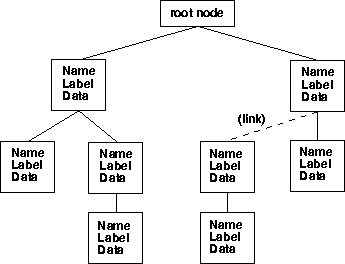
\includegraphics[scale=0.5]{img/cgns.png}
\caption{Example CGNS tree-like structure.}
\end{figure}


\section{\label{upgrades}Description of the new features}

All the upgrades were included in \stb using new parameters, added to the dictionary. The program still
uses the steering file. A parameter determines whether the new features or the old ones are used.
First are described the new parameters and features, then will be describe the issues encountered and the answers given for each format.

\subsection{Modifications in \stb's main program}

The following table describes the new parameters available for the steering file:\\

\begin{tabular}{p{140pt}@{ : }p{200pt}}
\textbf{CONVERTER} & (Boolean) If true then use the new features.\\
\textbf{DEBUG} & (Boolean) If true display debug informations.\\
\textbf{SELAFIN IN DOUBLE PRECISION} & (Boolean) If true the \slf file will be read/written in double precision.\\
\textbf{INPUT FILE FORMAT} & (String) The format of the input file, \med, \unv, \slf.\\
\textbf{OUTPUT FILE FORMAT} & (String) The format of the output file, \med, \unv, \slf, \vtk.\\
\textbf{INPUT FILE} & (String) The name of the input file.\\
\textbf{BOUNDARY FILE} & (String) The name of the boundary file if it exists (optional).\\
\textbf{LOG FILE} & (String) The name of the complementary file, for the \unv format only.\\
\textbf{OUTPUT FILE} & (String) The name of the output file.\\
\textbf{OUTPUT BOUNDARY FILE} & (String) The name of the output boundary file if it exists (optional).\\
\textbf{OUTPUT LOG FILE} & (String) The name of the output complementary file, for the \unv format only.\\
\end{tabular}

The program works in two steps:
\begin{itemize}
\setlength{\itemsep}{1pt}
\setlength{\parskip}{0pt}
\setlength{\parsep}{0pt}
\item First the file is read and the mesh object structure is filled in.
\item The information from the mesh object structure are written into the output file.
\end{itemize}

All the format's functions (read/write) are contained in the file \verb+conv_+\textit{format}\verb+.f+ (where \textit{format} stands for \slf, \med, \ldots).\\

The table below shows which conversions are possible:

\begin{center}
\begin{tabular}{|l||*{5}{c|}}
\hline
\backslashbox{Input}{Output}  & \slf    & \med      & \unv      & \cgns     & \vtk    \\
\hline
\hline                                                          
\slf     & X         & \checked & \checked & \checked & \checked \\
\hline                                                         
\med     & \checked & X        & \checked & \checked & \checked \\
\hline                                                         
\unv     & \checked & \checked & X        & \checked & \checked \\
\hline                                                         
\cgns    & \checked & \checked & \checked & X        & \checked \\
\hline
\end{tabular}\\
\checked : Available, X : Unauthorized
\end{center}

The \unv format is the only format that can not manage results. It only contains the mesh and the colors.

\stb handles distributed meshes only for \med and \slf format.

Some formats use a file for each time step for the results file, this is the case for the \vtk format.

Instead of running \stb with a steering a script, named \verb+runStbtel.py+, has been created in order to launch the converter in a one-line-command. This script is written in \textbf{Python 2.6}.

Here is the way it works (To see to following message run \verb+runStbtel.py --help+):
\begin{verbatim}
Usage: runStbtel.py input-file-name -o output-file-name [options]
Example: runStbtel.py coarse.slf -b coarse.cli -o coarse.med --debug
Where coarse.slf is the mesh in SELAFIN fornat,
      coarse.cli is the boundary conditions file and
      coarse.med the converted mesh in MED format.

Options:
  -h, --help            show this help message and exit
  -o OUTPUTFILE, --output-file=OUTPUTFILE
                        name of the output file also defines the output format
  -b BOUNDARYFILE, --boundary-file=BOUNDARYFILE
                        name of the output file
  -l LOGFILE, --log-file=LOGFILE
                        name of the log file
  -n NDOMAINS, --ndomains=NDOMAINS
                        number of sub-domains of the distributed mesh
  -s, --silent          disable stbtel output informations
  -t, --temporary-folder
                        keep stbtel temporary folder and the temporary
                        steering file
  --selafin-double-precision
                        state that the selafin file is in double precision
  --debug               enable debug mode
\end{verbatim}

The conversion of all the files of a distributed mesh in one run is only available in the python script.

\subsection{The mesh object structure}

Here is a description of the object's structure that is used by the converter.
This object makes it easier to add new formats, for each format only two functions
will be needed one to fill the mesh object by reading the file and one writing the file using the mesh object's data. 
A similar object is used in the \bief library to store mesh information. 
This object is used as a common ground between all the formats handled by the converter.

\begin{description}
\setlength{\itemsep}{1pt}
\setlength{\parskip}{0pt}
\setlength{\parsep}{0pt}
\item[Common Block]
\item[title] Name of the mesh.
\item[description] Description of the mesh (only \med).
\item[ndim] Dimension of the domain (2 or 3).
\item[nelem] Number of elements.
\item[npoin] Number of nodes.
\item[ndp] Number of points per element.
\item[type\_elem] Type of element (triangle, quadrilateral, tetrahedron, prism).
\item[nptfr] Number of boundary nodes.
\item[ib] Table of 10 integers: ib(10) (only used for \slf).
\item[ikles] Connectivity table: ikles(nelem*ndp). 
\item[ipobo] Flag for boundary node: ipobo(npoin).
\item[x] x coordinates: x(npoin).
\item[y] y coordinates: y(npoin).
\item[z] z coordinates: z(npoin).
\item[namecoo] Name of the coordinates: namecoo(ndim).
\item[unitcoo] Unit of the coordinates: unitcoo(ndim).
\item[knolg] Global number of point: knolg(npoin).
\item[Results information]
\item[nvar] Total number of variables.
\item[namevar] Name of the variables: namevar(maxvar).
\item[unitvar] Unit of the variables: unitvar(maxvar).
\item[timestep] Number of time steps.
\item[times] Table containing for each time step its value in seconds: times(timestep).
\item[res] Results for all the time steps and all the variables: res(timestep,nvar,npoin).
\item[Families information]
\item[nfam] Number of families.
\item[idfam] id of the family: idfam(nfam).
\item[valfam] Value of each family: valfam(nfam).
\item[namefam] Name of each family: namefam(nfam).
\item[ngroupfam] Number of group of each family: ngroupfam(nfam).
\item[groupfam] Group of each families: groupfam(nfam,10).
\item[Boundary information]
\item[nbor] Local number of each boundary node: nbor(nptfr).
\item[libor] Value of each boundary node: libor(nptfr).
\item[\estel second element type information]
\item[nelem2] Number of elements.
\item[ndp2] Number of points per element.
\item[type\_elem2] Type of element.
\item[ikles2] Connectivity table: ikles2(nelem*ndp).
\item[Color information]
\item[color] Color of a node: color(npoin).
\item[ncolor] Color of an element: ncolor(nelem).
\item[ncolor2] Color of an element (\estel's second element): ncolor2(nelem2).
\end{description}


\subsection{\slf}

The code is implemented following the \bief library standards as much as possible. Three subroutines are used to read the 
mesh information \verb+readgeo1+, \verb+readgeo2+, \verb+readgeo3+. But they do not read the title, the variable information
nor the result information. The functions \verb+lit/ecri2+ of the \bief are used to read and write the extra information.
The \verb+readgeo+ functions contain an optional parameter in order to handle double precision real.
But in Fortran for the optional parameter to work, a function has to be declared in an interface and the function
in which it is called must contain the line \verb+use module+ which calls the interface.

When the results part of the \slf file is reached, the results table (\textbf{res} in mesh object) cannot be allocated because the number of time steps is unknown at this stage. 
To compute this value a quick read trough the rest of the file is carried out in order to count the number of records.
The file is then rewound, the results table can now be allocated and filled in.

Because the function rewind causes problems with some machines/compilers (for instance with GCC-4.1.2) the file is closed and re-opened instead.

An extra file which contains the read/write functions for the boundary file has been added.

Note that the title is set to have a length of 72 characters in the \bief library but it is defined with a length of 80 in the \tecplot plug-in and the \verb+sel2vtk+ program.

\subsection{\med}

Families are used to assign a value to a point. They can also be used to represent colors or boundary conditions.
A family and a group is created for each value (\verb?lihbor*100+liubor*10+livbor?). \verb+lihbor+, \verb+liubor+ and \verb+livbor+ are the first three columns of the
boundary file. \verb+hbor+, \verb+ubor+, \verb+vbor+ cannot be stored because they are defined as floating points whereas the family's value can only be an integer.

As a node only belongs to one family, both color and boundary conditions cannot be handled.
Currently either color or boundary features are handled, with priority to the boundary conditions if both are 
available.

The zero family has to be defined in \med as it is the default family.

\med allows to manipulate vectors (the \verb+ifvector_+ function from \verb+m_med.f+ in the \bief library defines which 
variable is a vector). Those variables are then merged into one. For example the variables \verb+VITESSE_U_+ and 
\verb+VITESSE_V_+ becomes \verb+vitesse_*_+ which is a variable with two components.

In \med format results values can be declared for elements or nodes but in \slf format this is only possible for nodes.

There is a rounding error of the time step value in a \med file generated by \tel. It might come from the
conversion from single to double precision in \tel. This error could not be fixed in the converter, but \sal seems to correct it with a working rounding.

\subsection{\unv}

\bief library designed functions \verb+lit/ecri2+ cannot be used for the \unv format (ASCII) because they are made for reading/writing binary files only.
Currently the \textbf{ikles/color} tables are allocated with a size of the total numbers of element (2D and 3D elements) and are then resized.
Memory would be optimized by reading the file twice, first to compute the number of element of each type and
then to read the data. But it would double the reading time.

The \unv has a lot of sections available but only a few are used in \estel. For example \sal uses another section to determine the name of the groups and families.
It would be interesting to include this section in the converter because currently groups/families are named
using their values. They have to be changed manually in \sal. Families names also exist in the log file
but some of those families have the same value which does not fit the description of the families in \med.

\subsection{\vtk}

Three different ways were selected to handle \vtk files:

\begin{itemize}
\item Using the existing \verb+sel2vtk+ program. But it is old (2005) and it may not be maintained in the future.
\item Using the \vtk library. But the library is really huge because it contains the \vtk viewer too.
It is written in C++, and is therefore complicated to wrap it in Fortran.
\item Using the \verb+lib_vtk_io+ library. Unfortunately it is not completed and contains only the functions to write a \vtk file.
The reading functions have not been developed to this day.
\end{itemize}

In \stb the library \verb+lib_vtk_io+, developed by Stefano Zaghi and colleagues
(\url{http://sites.google.com/site/stefanozaghi/lib\_vtk\_io}), is used.

It was chosen because it contains enough functionalities and is still maintained. 
It is written in Fortran which makes it easy to include in \stb and to use.

A few parameters in the function \verb+open+ were in Fortran 2003. They were removed to comply with
Fortran 90 standard. The code was also re-indented to fit Fortran line length standard.

\vtk only supports 3D meshes, a table of zeros was created for the z coordinates in 2D.
For the result information a file has to be created at each time step, which name should be 
\verb+outfile+\textit{timestep}\verb+.vtk+. But due to the fact that the time step is a real number, a continuous numbering is used instead. 

\subsection{\cgns}
Some issues arise with the installation of \hdf on some clusters.
Therefore the \cgns library will be used without \hdf. 

The last stable version of \cgns (3.1.3), released in March 2011 is not currently handled by neither \textbf{ParaView} nor \tecplot. Therefore
the previous stable version (2.5.5) is plugged in \stb. The installation of this version cannot find \verb+gfortran+, but only \verb+f90+. 
A link from \verb+f90+ to \verb+gfortran+ is necessary.

In \cgns strings all have a length of 32, the mesh title is then much smaller than for other formats.
\cgns mostly uses defined variables. Most \tel variables are represented but a function
to associate each \tel variable to a \cgns one is required. A way around is to use user-defined variables, but the variable's unit cannot be defined.



\subsection{Omitted formats}

Three other formats have been deliberately omitted \tecplot, \textbf{Plot3d}, \textbf{XDMF}.

The \tecplot format is handled by a plug-in reading \slf files
to \tecplot (it can be found in \tel svn repository). A library \verb+tecio.f+ also exists, which was developed within
the \tecplot community. 

The \textbf{Plot3d} format is only used for structured grid and cannot handle \tel meshes.
If the nodes can be defined, the connectivity is only set by the structured grid's informations.
There is no standard for the variables, which is handled differently by each pre-\&post-processing software.

The \textbf{XDMF} format is a combination of \hdf and XML formats.
It is used by HR Wallingford. The website (\url{http://www.xdmf.org}) does not 
give enough informations to add this format to \stb.

\section{\label{improvment}Possible future development}

\begin{itemize}
\setlength{\itemsep}{1pt}
\setlength{\parskip}{0pt}
\setlength{\parsep}{0pt}
\item Coding a \slf library to standardise the format. This way changes would be transparent to users.
The \bief library already performs most of the operations but it would need to be completed.
\item Selecting the variables in \stb in order to reduce the file size.
\item Converting from \slf 2D with a number of layers to \slf 3D and building the boundary file.
\item Adding to \slf format information concerning the precision of the reals by using one of the available ten integers.
The additional format \textbf{SELAFIND} could then be dropped.
\end{itemize}

\section{Conclusion}
\stb is now able to convert from \med, \slf, \unv, \cgns  to \med, \slf, \unv, \cgns, \vtk, which allows to use larger variety of pre-\&post-processing tools.
None of the formats contain all the information of the mesh object structure. This explains why some data are lost during a conversion.
For example the \slf format cannot handle families/colors. No format is able to integrate
the boundary file even if the \med format almost does it.
The \med format cannot contain both colors and boundaries. 
Moreover the fact that all the results are contained in one file makes the size of the table \verb+res+ increasing 
quickly as a function of the number of time steps, the number of points and the number of variables. This table defines the memory threshold of \stb.
The development of a new format (\textbf{SELAFIN2}) should 
take into account all those remarks. 

\newpage
\appendix
\appendixpage


\section{Installation of \stb external library}

The installation of the external library, \hdf, \med, \cgns can be done using this script. The example here is for an IBM POWER7 cluster:
\codebash{img/install.sh}
Here are some examples of how to use the script :

\begin{verbatim}
# install only hdf5
./install.sh HDF5
# install only MED hdf5 is needed
./install.sh MED
install only cgns
./install.sh CGNS
# install all the above
./install.sh ALL
\end{verbatim}

\section{Installation of \stb}

In \stb \verb+if defined+ statement (macros) are used to handle external libraries. Preprocessing is required while compiling.
To handle \verb+ifdef+ macro two solutions are available :
\begin{itemize}
\item Changing the extension of the file containing the macro by .F (resp. .F90) which will launch the preprocessor by default.
\item Adding the following options to the compiler:
\begin{itemize}
\setlength{\itemsep}{1pt}
\setlength{\parskip}{0pt}
\setlength{\parsep}{0pt}
\item For gnu compiler (gfortran): \verb+-x f95-cpp-input+
\item For pgi compiler (pgf90): \verb+-Mpreprocess+ 
\item For intel compiler (ifort): \verb+-cpp+ 
\item On IBM Bluegene/Power7 (xlf): \verb+-qsuffix=cpp=f+ and add \verb+-WF,+ before \verb+-D+
\end{itemize}
These options must be added even if no external libraries are used.
\end{itemize}

Adding external library, if available, is done as follows in
\tel \verb+systel.ini+:
\begin{itemize}
\setlength{\itemsep}{1pt}
\setlength{\parskip}{0pt}
\setlength{\parsep}{0pt}
\item For \med  : add \verb+-DHAVE_MED -Imed_direcoty/include+ to the compiler 
options (\verb+FC_OPT_OTHERS+).\\
\verb!-lm -lz -lstdc++ -Lhdf5_directory/lib -lhdf5 -Lmed_directory/lib -lmed! to the linker 
options (\verb+LK_LIB_SPECIAL+).
\item For \cgns  : add \verb+-DHAVE_CGNS -Icgns_direcoty/include+ to the compiler 
options (\verb+FC_OPT_OTHERS+).\\
\verb+-Lcgns_directory/lib -lcgns+ to the linker options (\verb+LK_LIB_SPECIAL+).
\end{itemize}

\section{Validation cases}

A few cases were added under the sub-folder \verb+converter+ in \stb validation folder.
Below is the list of the folders added.

\subsection{001\_unv}

This folder contains tests for the \unv format:-
\begin{itemize}
\item \textit{stb\_coornov2010\_fin.cas} is a conversion of a 2D mesh (see Fig. \ref{coornov}) 
from \unv to \med format. 
\item \textit{stb\_coarse.cas} is a conversion of a 3D mesh containing triangles and tetrahedrons from
\unv to \med format.
\item \textit{stb\_geo\_riogrande.cas} is a conversion of a 2D representation of the Rio Grande river 
from \slf to \unv format.
\end{itemize}
The \unv format contains colors that are conserved as groups of nodes/elements 
in \med format but are lost in \slf format.

\begin{figure}[ht]
  \centering
  \includegraphics[scale=0.5]{img/coornov.jpg}
  \caption{A basic 2d mesh.}
  \label{coornov}
\end{figure}

\subsection{002\_med}

This folder contains tests for the \med format:-
\begin{itemize}
\item \textit{stb\_r2d\_malpasset.cas} is a conversion of a 2D representation of the Malpasset dam-break (see Fig. \ref{malpasset}) with results 
from \med to \slf format.
\item \textit{stb\_r3d\_malpasset.cas} is a conversion of a 3D representation of the Malpasset dam-break with results 
from \med to \slf format.
\end{itemize}
All groups information that were inside the \med file are lost in the \slf format.

\begin{figure}[ht]
  \centering
  \includegraphics[scale=0.5]{img/malpasset.jpg}
  \caption{The Malpasset dam-break mesh}
  \label{malpasset}
\end{figure}

\subsection{003\_selafin}

This folder contains tests for the \slf format:-
\begin{itemize}
\item \textit{stb\_geo\_malpasset.cas} is a conversion of a 2D representation of the Malpasset dam-break without results 
from \slf to \med format.
\item \textit{stb\_r2d\_malpasset.cas} is a conversion of a 2D representation of the Malpasset dam-break with results 
from \slf to \med format.
\item \textit{stb\_r3d\_malpasset.cas} is a conversion of a 3D representation of the Malpasset dam-break with results 
from \slf to \med format.
\end{itemize}
The boundary condition file information are converted into groups in the \med file. 
But only the first three columns of the boundary file are conserved the rest is lost.

\subsection{004\_vtk}

This folder contains tests for the \vtk format:-
\begin{itemize}
\item \textit{stb\_geo\_riogrande.cas} is a conversion of a 2D representation of the Rio Grande river 
from \slf to \vtk format.
\item \textit{stb\_r2d\_riogrande.cas} is a conversion of a 2D representation of the Rio Grande river 
with results from \slf to \vtk format.
\end{itemize}
The time step values are lost during the conversion they are replaced by the time-step number.

\subsection{005\_cgns}

This folder contains tests for the \cgns format:-
\begin{itemize}
\item \textit{stb\_geo\_malpasset.cas} is a conversion of a 2D representation of the Malpasset dam-break without results 
from \slf to \cgns format.
\item \textit{stb\_r2d\_malpasset.cas} is a conversion of a 2D representation of the Malpasset dam-break with results 
from \slf to \cgns format.
\end{itemize}

\subsection{006\_distributed\_mesh}

This folder contains tests for the \unv format.
\verb+006_distributed_mesh+ contains a script for the conversion of a distributed mesh
in \slf format into \med format. This test can only work with the \verb+runStbtel.py+ python script.

\begin{thebibliography}{9}
\bibitem{telemac}
  Telemac System,
  EDF,
  \url{www.opentelemac.org}.
\bibitem{salome}
  Salome,
  EDF,
  \url{www.salome-platform.org}.
\bibitem{paraview}
  ParaView,
  Kitware,
  \url{www.paraview.org}.
\bibitem{visit}
  VisIt,
  Lawrence Livermore National Laboratory,
  \url{visit.llnl.gov}.
\bibitem{med}
  MED,
  EDF,
  \url{www.code-aster.org/outils/med}.
\bibitem{unv}
  UNV,
  I-DEAS.
\bibitem{vtk}
  VTK,
  Kitware,
  \url{www.vtk.org}.
\bibitem{cgns}
  CGNS,
  CGNS Steering Committee,
  \url{cgns.sourceforge.net}.
\end{thebibliography}
%-----------------------------------------------------------
\end{document}
